\documentclass[a4paper,titlepage,12pt]{article}
\usepackage[utf8]{inputenc} %Make sure all UTF8 characters work in the document
\usepackage{listings} %Add code sections
\usepackage{color}
\usepackage{graphicx}
\usepackage{titling}
\usepackage{textcomp}
\usepackage{tabularx}
\usepackage[hyphens]{url}
\usepackage[bottom]{footmisc}
\usepackage[yyyymmdd]{datetime}
\usepackage[figurename=Figur]{caption}
\definecolor{listinggray}{gray}{0.9}
\definecolor{lbcolor}{rgb}{0.9,0.9,0.9}
\usepackage{longtable}
\usepackage{pbox}
\usepackage{booktabs}

%Set page size
\usepackage{geometry}
\geometry{margin=3cm}
\usepackage{parskip} 

\renewcommand{\dateseparator}{-}
\renewcommand{\contentsname}{Innehållsförteckning}


%%%%%%%%%%%%%%%%%%%%%%%%%%%%%%%
% Header and footer
%%%%%%%%%%%%%%%%%%%%%%%%%%%%%%%
\usepackage{fancyhdr}
\pagestyle{fancy}

\lhead{
\includegraphics[width=0.15\linewidth]{../images/logo_full.png}}
\chead{Kravspecifikation för sexbent robot}
\rhead{\today}
\setlength\headheight{26pt} 

\lfoot{TSEA29 --- KMM \\ LIPS Kravspecifikation}
\rfoot{Grupp 9 \\ LiTHe Hex}

\pretitle{%
    \begin{center}
        \LARGE
        
\includegraphics[width=6cm]{../images/logo_full.png}\\[\bigskipamount]
}

\posttitle{\end{center}}

\newcounter{reqNr}
\setcounter{reqNr}{0}
\newcommand{\nextReqNr}{\stepcounter{reqNr}\arabic{reqNr}}

\newcounter{reqNrII}
\setcounter{reqNrII}{16}
\newcommand{\nextReqNrII}{\stepcounter{reqNrII}\arabic{reqNrII}}

\newcommand{\newContent}[1] {\pbox{5cm}{Nytt innehåll i \arabic{reqNr}\\#1}}
\newcommand{\newRequirement}[1] {\pbox{5cm}{Nytt krav \\#1}}

\begin{document}

    \title{\LARGE
        \textbf{Kravspecifikation för sexbent robot} \\
        \vspace*{0.5\baselineskip}
        \large
        Redaktör Frans Skarman \\
        Grupp 9 \\
        \small
        \vspace*{0.5\baselineskip}
        Version 0.2}

    \date{\today}

	\maketitle
	\newpage

	\tableofcontents
	
	\newpage
	
	\begin{center}

		%%%%%%%%%%%%%%%%%%%%%%%%%%%%%%%%%%%%%%%%%%%%%%%%%%%%%%%%%%%%%%%%%%%%%%%%%%%%%%%%%
		%						Medlemmar
		%%%%%%%%%%%%%%%%%%%%%%%%%%%%%%%%%%%%%%%%%%%%%%%%%%%%%%%%%%%%%%%%%%%%%%%%%%%%%%%%%

		\section*{Projektidentitet}
		Grupp 9, Ht 2016, LiTHe Hex

		Linköpings Tekniska Högskola, ISY

		\begin{table}[h]
			\begin{center}
				\begin{tabular}[pos]{ l l l }
					\textbf{Namn} & \textbf{Ansvar} & \textbf{E-post} \\ \midrule
					Emil Segerbäck & & emise935@student.liu.se \\ \midrule
					Frans Skarman & Dokumentansvarig & frask812@student.liu.se \\ \midrule
					Hannes Tuhkala & & hantu447@student.liu.se \\ \midrule
					Malcolm Vigren & Projektledare & malvi108@student.liu.se \\ \midrule
					Noak Ringman &  & noari093@student.liu.se \\ \midrule
					Olav Övrebö &  & olaov121@student.liu.se \\ \midrule
					Robin Sliwa &  & robsl733@student.liu.se \\
				\end{tabular}
			\end{center}
		\end{table}

		\centering
		\textbf{Kursansvarig}: Tomas Svensson Rum 3B:528 013--28 13 68 tomas.svensson@liu.se


		
		\newpage


		%%%%%%%%%%%%%%%%%%%%%%%%%%%%%%%%%%%%%%%%%%%%%%%%%%%%%%%%%%%%%%%%%%%%%%%%%%%%%%%%%
		%						Historik
		%%%%%%%%%%%%%%%%%%%%%%%%%%%%%%%%%%%%%%%%%%%%%%%%%%%%%%%%%%%%%%%%%%%%%%%%%%%%%%%%%

		\section*{Dokumenthistorik}
		\begin{table}[h]
			\begin{tabular}[pos]{ l l l l l }
				\textbf{Version} & \textbf{Datum} & \textbf{Utförda förändringar} 
				& \textbf{Utförda av} & \textbf{Granskad} \\ \midrule

				0.1 & 2016--09--07 & Första utkastet & Projektgruppen & Tomas Svensson \\ \midrule
				0.2  & 2016--09--09 & Andra utkastet & Projektgruppen & \\

			\end{tabular}
		\end{table}

	\end{center}

	%%%%%%%%%%%%%%%%%%%%%%%%%%%%%%%%%%%%%%%%%%%%%%%%%%%%%%%%%%%%%%%%%%%%%%%%%%%%%%%%%
	%						Inledning
	%%%%%%%%%%%%%%%%%%%%%%%%%%%%%%%%%%%%%%%%%%%%%%%%%%%%%%%%%%%%%%%%%%%%%%%%%%%%%%%%%

	\newpage

	\section{Inledning}
	I detta dokument beskrivs funktionaliteten produkten ska ha vid leverans. All funktionalitet har strukturerats i olika krav där det 
	blir tydligt om kravet är uppfyllt eller inte. Krav har olika nivåer där
	nivå 1 är ska-krav som måste ha uppfyllts vid leverans. Nivå 2 ses som bör-krav 
	och uppfylls i mån av tid.

	\subsection{Parter}
	Projektets beställare och kund är Tomas Svensson, lektor vid Linköpings tekniska högskola.
	Projektets producent är projektgrupp 9, bestående av 7 studenter från D-programmet, också vid 
	Linköpings tekniska högskola.
	\subsection{Syfte och mål}
	Syftet och målet med projektet är att utveckla en sexbent robot som själv
	kan navigera sig ut ur en labyrint. I labyrinten bör roboten även kunna ta 
	sig över hinder för att komma vidare. 
	\subsection{Bakgrundsinformation}
	För regler om uppbyggnad av labyrinten som roboten är tänkt att ta sig igenom, se
	Bilaga A:\ Banregler.

	%%%%%%%%%%%%%%%%%%%%%%%%%%%%%%%%%%%%%%%%%%%%%%%%%%%%%%%%%%%%%%%%%%%%%%%%%%%%%%%%%
	%						Översikt
	%%%%%%%%%%%%%%%%%%%%%%%%%%%%%%%%%%%%%%%%%%%%%%%%%%%%%%%%%%%%%%%%%%%%%%%%%%%%%%%%%

  \newpage
	\section{Översikt av systemet}
	Systemet ska innehålla tre enheter. En centralenhet för kommunikation med en dator, en motorikenhet
	som sköter hur benen rör sig samt en sensorenhet som tolkar sensordata. Centralenheten är även den enhet som
	tar beslut och kommunicerar med de andra enheterna. Se Figur. 1 för en översiktsbild av systemet.
	\begin{figure}[h]
		\centering
		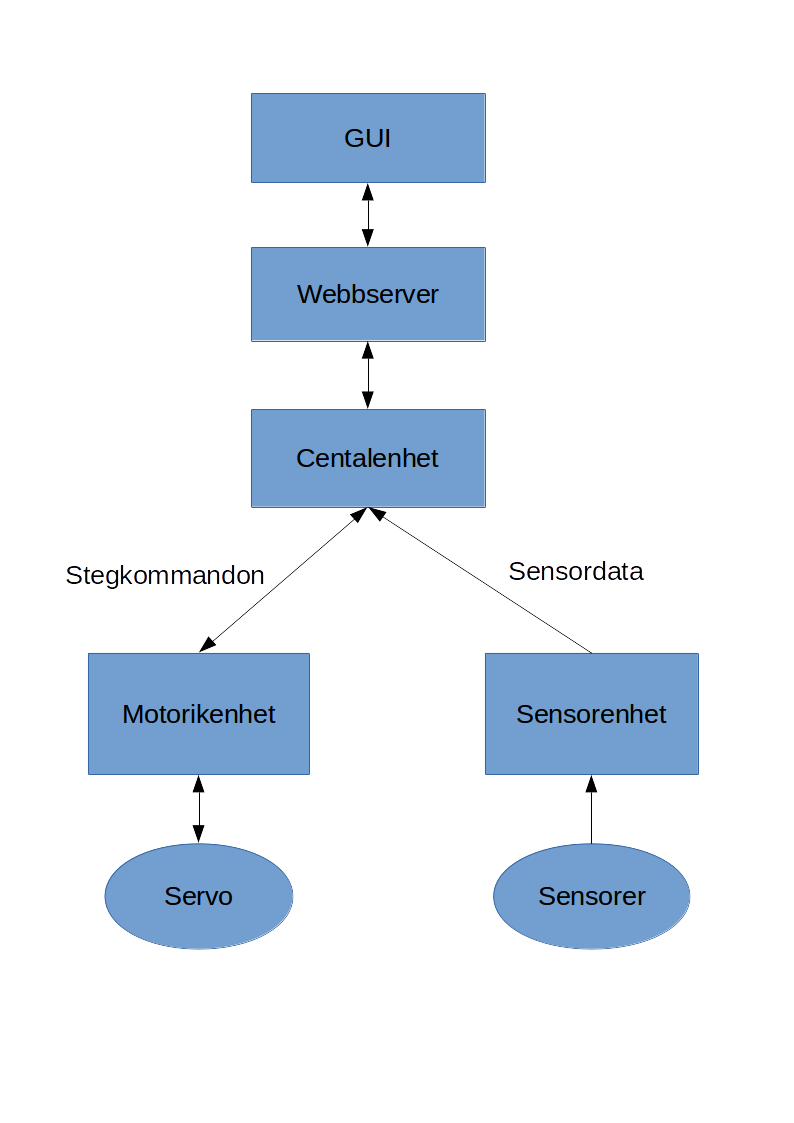
\includegraphics[width=0.5\linewidth]{../images/overview.png}
		\caption{Översikt av systemet\label{fig:overview}}
	\end{figure}

	\subsection{Grov beskrivning av produkten}
	Produkten är en sexbent robot som känner av sin omgivning och kan gå autonomt
	genom en bana samt styras manuellt.
	\subsection{Produktkomponenter}
	I leveransen ska det ingå en autonom sexbent robot med tillhörande GUI som kan användas för att 
	styra roboten manuellt. Även teknisk dokumentation och demonstration ingår. 
	\subsection{Beroenden  till andra system}
    För manuell styrning är roboten beroende av WiFi-kommunikation med en dator.
	\subsection{Ingående delsystem}
    De ingående delsystemen är:
    
    \begin{itemize}
        \item Centralenheten
        \item Motorikenheten
        \item Sensorenheten
    \end{itemize}
	\subsection{Avgränsningar}
	Roboten behöver inte klara mer avancerade former på labyrinten än de som beskrivs i Bilaga A:\ Banregler.
	\subsection{Generella krav på hela systemet}

	%Generella krav på systemet
	\begin{table}[h]
		\begin{tabularx}{\textwidth}{ c l X l }
			\textbf{Nr} & \textbf{Förändring} & \textbf{Kravtext} & \textbf{Prioritet} 
				\\ \midrule
			\nextReqNr{} & Original & Roboten ska ha ett autonomt läge. & Utgått
					\\ \midrule
	
			\arabic{reqNr}A & \newContent{2016--09--09} & Roboten ska ha ett autonomt läge där den kan ta
                              sig igenom en bana enligt banspecifikationen & 1
					\\ \midrule

			\nextReqNr{} & Original & Roboten ska ha en knapp med vilken man startar 
				dess autonoma läge. & 1
				\\ \midrule

			\nextReqNr{} & Original & Roboten ska kunna styras med dator 
				via WiFi-länk. & 1
				\\ \midrule
		
			\nextReqNr{} & Original & Robotens sensordata ska gå att läsa 
				med dator via WiFi & 1
				\\ \midrule

			\nextReqNr{} & Original & Robotens styrbeslut ska gå att läsa 
				med dator via WiFi & 1
                \\ \midrule
      
      % needs a new number!
			\nextReqNr{} & \newRequirement{2016--09--09} & Via WiFi ska roboten kunna reagera på förljande
                              kommandon: framåt, bakåt, stop, framåt vänster,
                              framåt höger, rotera vänster, rotera höger,
                              autonomt läge av och på & 1
                \\ \midrule

            \nextReqNrII{} & \newRequirement{2016--09--09} & Gränssnitten
            mellan delsystemen ska vara noggrannt specificerad i
            designspecifikationen och den tekniska dokumentationen. & 1
                \\ \midrule

            \nextReqNrII{} & \newRequirement{2016--09--09} & Varje delsystem
            ska innehålla minst en processor. & 1
				\\ \bottomrule
		\end{tabularx}
	\end{table}

	%%%%%%%%%%%%%%%%%%%%%%%%%%%%%%%%%%%%%%%%%%%%%%%%%%%%%%%%%%%%%%%%%%%%%%%%%%%%%%%%%
	%						Centralenhet
	%%%%%%%%%%%%%%%%%%%%%%%%%%%%%%%%%%%%%%%%%%%%%%%%%%%%%%%%%%%%%%%%%%%%%%%%%%%%%%%%%
	\section{Delsystem centralenhet}
	Centralenheten ska styra alla andra delsystem i konstruktionen samt sköta
	kommunikation till omvärlden via WiFi. Denna ska utgöras av en Raspberry
	Pi, som är en passande dator då den har inbyggd hårdvara för WiFi. Den har 
	också ett operativsystem gör att programmering kan ske på en relativt hög nivå.

	\newpage

	\subsection{Krav}
	\begin{table}[h]
		\begin{tabularx}{\textwidth}{c l X l}
			\textbf{Nr} & \textbf{Förändring} & \textbf{Kravtext} & \textbf{Prioritet} 
				\\ \midrule

			\nextReqNr{} & Original & Centralenheten ska kunna kommunicera 
				med en dator via WiFi. & 1
				\\ \midrule

			\nextReqNr{} & Original & Centralenheten ska kunna ta emot och 
				behandla data från sensorenheten.& Utgått
				\\ \midrule
			\arabic{reqNr}a & \newContent{2016--09--09} & Centralenheten ska kunna ta emot och 
				behandla data från sensorenheten.& 1
				\\ \midrule

			\nextReqNr{} & Original & Centralenheten ska kunna ta emot från, 
				behandla och skicka information till motorikenheten. & Utgått
				\\ \midrule
			\arabic{reqNr}a & \newContent{2016--09--09} & Centralenheten ska kunna ta emot från
				 och skicka information till motorikenheten. & 1
				\\ \midrule

			\nextReqNr{} & Original & Centralenheten ska kunna upptäcka hinder. & 2
			\\ \midrule

			\nextReqNrII{} & \newRequirement{2016--09--09} & Centralenheten ska kunna använda
			datan från sensor- och motorikenheten för att navigera i banan.  & 1
		\end{tabularx}
	\end{table}



	%%%%%%%%%%%%%%%%%%%%%%%%%%%%%%%%%%%%%%%%%%%%%%%%%%%%%%%%%%%%%%%%%%%%%%%%%%%%%%%%%
	%						Motorikenhet
	%%%%%%%%%%%%%%%%%%%%%%%%%%%%%%%%%%%%%%%%%%%%%%%%%%%%%%%%%%%%%%%%%%%%%%%%%%%%%%%%%

	\section{Delsystem motorikenhet}
	Motorikenhetens syfte är att ta data om vilket håll roboten ska gå och styra benen enligt de
	instruktionerna. Den ska bestå av en AVR-processor som tar kommandon från styrdatorn och skickar
	servopositioner till de individuella servona. Enheten ska även kunna skicka data om underlagets
	höjd till centralenheten.

	\subsection{Krav}
	\begin{table}[h]
		\begin{tabularx}{\textwidth}{c l X l}
			\textbf{Nr} & \textbf{Förändring} & \textbf{Kravtext} & \textbf{Prioritet} 
				\\ \midrule

			\nextReqNr{} & Original & Motorikenheten ska möjliggöra rörelse framåt och 
				bakåt samt rotation. & 1
				\\ \midrule

			\nextReqNr{} & Original & Motorikenheten ska ge roboten två olika gånglägen,
				ett där roboten går 
				snabbt och ett där roboten går med högre precision.& 2
				\\ \midrule

			\nextReqNr{} & Original & Motorikenheten ska kunna skicka data om höjden 
				på underlaget till centralenheten. & 2
				\\ \midrule

			\nextReqNr{} & Original & Motorikenheten ska möjliggöra kliv över hinder 
				beskrivna i Bilaga A:\
  				Banregler. & 2
				\\ \midrule

			\nextReqNr{} & Original & Motorikenheten ska möjliggöra rörelse åt höger 
				och vänster. & 2 

		\end{tabularx}
	\end{table}


	%%%%%%%%%%%%%%%%%%%%%%%%%%%%%%%%%%%%%%%%%%%%%%%%%%%%%%%%%%%%%%%%%%%%%%%%%%%%%%%%%
	%						Sensorer
	%%%%%%%%%%%%%%%%%%%%%%%%%%%%%%%%%%%%%%%%%%%%%%%%%%%%%%%%%%%%%%%%%%%%%%%%%%%%%%%%%
	\section{Delsystem sensorenhet}
	Sensorenheten är en mikrodator som ska läsa data från sensorer för att sedan skicka 
	den vidare till centralenheten. Sensorer är avståndsmätare och eventuella extra sensorer 
	för att detektera hinder.

	\subsection{Krav}
	\begin{table}[h]
		\begin{tabularx}{\textwidth}{c l X l}
			\textbf{Nr} & \textbf{Förändring} & \textbf{Kravtext} & \textbf{Prioritet} 
				\\ \midrule

			\nextReqNr{} & Original & Sensorenheten ska kunna tolka avstånds- mätarnas data. & 1
				\\ \midrule

			\nextReqNr{} & Original & Sensorenheten ska kunna kommunicera med 
				centralenheten. & 1

		\end{tabularx}
	\end{table}

	%%%%%%%%%%%%%%%%%%%%%%%%%%%%%%%%%%%%%%%%%%%%%%%%%%%%%%%%%%%%%%%%%%%%%%%%%%%%%%%%%
	%						Grafiskt användargränssnitt
	%%%%%%%%%%%%%%%%%%%%%%%%%%%%%%%%%%%%%%%%%%%%%%%%%%%%%%%%%%%%%%%%%%%%%%%%%%%%%%%%%
    \section{Grafiskt användargränssnitt}
    På centralenheten ska en webserver köras. Webserverns syfte är att
    tillhandahålla ett grafiskt användargränssnitt där användaren kan skicka
    styrkommandon och läsa sensordata.
	\subsection{Krav}
	\begin{table}[h]
      \begin{tabularx}{\textwidth}{c l X l}
        \textbf{Nr} & \textbf{Förändring} & \textbf{Kravtext} & \textbf{Prioritet} 
        \\ \midrule

        \nextReqNr{} & Original & Användaren ska kunna styra roboten från
                                  det grafiska gränssnittet. & 1
        \\ \midrule

        \nextReqNr{} & Original & Användaren ska kunna läsa sensordata i det
                                  grafiska gränssnittet. & 1

      \end{tabularx}
	\end{table}

	%%%%%%%%%%%%%%%%%%%%%%%%%%%%%%%%%%%%%%%%%%%%%%%%%%%%%%%%%%%%%%%%%%%%%%%%%%%%%%%%%
	%						Extrakrav
	%%%%%%%%%%%%%%%%%%%%%%%%%%%%%%%%%%%%%%%%%%%%%%%%%%%%%%%%%%%%%%%%%%%%%%%%%%%%%%%%%
	\section{Krav på vidareutveckling}
	Roboten ska kunna utvecklas vidare för att få en mer avancerad styrning av benen, 
	den ska exempelvis kunna gå snabbare och jämnare. Koden och hårdvaran ska också vara
	konstruerad på ett sådant sätt att det ska gå att programmera roboten för
	kartläggning av ett utrymme.

	\section{Ekonomi}

	\begin{table}[h]
		\begin{tabularx}{\textwidth}{c l X l}
			\textbf{Nr} & \textbf{Förändring} & \textbf{Kravtext} & \textbf{Prioritet} 
			\\ \midrule
			
			\nextReqNr{} & 2016--09--09 & Efter godkänd projektplan får
            maximalt 1120 arbetstimmar användas på projektet. & 1
		\end{tabularx}
	\end{table}

	\section{Leveranskrav och delleveranser}
	Delleveranser är leverans av projektplan, leverans av designspecifikation 
	samt slutleverans. Slutleveransen består av en presentation av projektet, 
	demonstration av roboten i autonomnt och manuellt läge i form av en tävling,
	samt överlämning av kod, hårdvara och dokumentation.

	\subsection{Krav}
	\begin{table}[h]
		\label{tab:Krav leverans}
		\begin{tabularx}{\textwidth}{|c|l|X|l|}
			\hline
			\textbf{Nr} & \textbf{Förändring} & \textbf{Kravtext} & \textbf{Prioritet} 
				\\ \hline

			\nextReqNr & Tillagd 2016-09-09 & Första versionen av
                designspecifikationen ska vara inlämnad till handledaren senast
                2016-11-01. & 1
				\\ \hline

			\nextReqNr & Tillagd 2016-09-09 & Slutgiltig designspecifikation
                ska vara godkänd av handledaren senast 2016-11-04. & 1
				\\ \hline
                
			\nextReqNr & Tillagd 2016-09-09 & Slutpresentation av projektet ska
            ske 2016-12-19. & 1
				\\ \hline

			\nextReqNr & Tillagd 2016-09-09 & Slutpresentationen ska bestå av
            ett bildspel på projektor. & 1
				\\ \hline

			\nextReqNr & Tillagd 2016-09-09 & Slutpresentationen ska ha en
            längd mellan 15-20 minuter. & 1
				\\ \hline

			\nextReqNr & Tillagd 2016-09-09 & Demonstrationen av projektet ska
            bestå av tävlingar med andra grupper som gjort projekt med sexbent
            robot, och ska äga rum 2016-12-20. Tävlingsregler beskrivs i Bilaga
            A: Ban- och regelspecifikation. & 1
				\\ \hline

			\nextReqNr & Tillagd 2016-09-09 & Senast tre dagar innan
                presentationen av projektet ska den tekniska dokumentationen
                samt användarhandledning vara inlämnad till beställaren. & 1
				\\ \hline

			\nextReqNr & Tillagd 2016-09-09 & Efterstudien ska vara inlämnad
            till beställaren senast 2016-12-22. & 1
				\\ \hline

		\end{tabularx}
	\end{table}
	
	\section{Dokumentation}
    Följande dokumentation inkluderas i projektet:
    \begin{itemize}
		\item Tidplan 
		\item Systemskiss 
		\item Projektplan
		\item Teknisk dokumentation 
		\item Användarhandledning 
        \item Designspecifikation
        \item Efterstudie
    \end{itemize}

	\subsection{Krav}
	\begin{table}[h]
		\label{tab:Krav dokumentation}
		\begin{tabularx}{\textwidth}{|c|l|X|l|}
			\hline
			\textbf{Nr} & \textbf{Förändring} & \textbf{Kravtext} & \textbf{Prioritet} 
				\\ \hline

			\nextReqNr & Tillagd 2016-09-09 & Alla dokument ska vara skrivna
            enligt LIPS-mallar. & 1
				\\ \hline

		\end{tabularx}
	\end{table}

\end{document}



%%%%%%%%%%%%%%%%%%%%%%%%%%%%%%%%%%%%%%%%%%%%%%%%%%%%%%%%%%%%%%%%%%%%%%%%%%%%%%%%%
%						Templates
%%%%%%%%%%%%%%%%%%%%%%%%%%%%%%%%%%%%%%%%%%%%%%%%%%%%%%%%%%%%%%%%%%%%%%%%%%%%%%%%%

\iffalse{}
	\begin{table}[h]
		\begin{tabularx}{\textwidth}{c l X l}
		\textbf{Nr} & \textbf{Förändring} & \textbf{Kravtext} & \textbf{Prioritet} 
		\\ \midrule
	
		1 & Original & Roboten ska autonomt kunna navigera sig igenom tvävlingsbanan & 1
		\end{tabularx}
	\end{table}
\fi
